\documentclass[journal, a4paper]{IEEEtran}

% some very useful LaTeX packages include:
\usepackage[brazil]{babel}
\usepackage[utf8x]{inputenc}
\usepackage{amsmath}
\usepackage{float}
\usepackage{mathtools}
\usepackage{natbib}
%\usepackage{multicol, blindtext}

%\usepackage{cite}      % Written by Donald Arseneau
                        % V1.6 and later of IEEEtran pre-defines the format
                        % of the cite.sty package \cite{} output to follow
                        % that of IEEE. Loading the cite package will
                        % result in citation numbers being automatically
                        % sorted and properly "ranged". i.e.,
                        % [1], [9], [2], [7], [5], [6]
                        % (without using cite.sty)
                        % will become:
                        % [1], [2], [5]--[7], [9] (using cite.sty)
                        % cite.sty's \cite will automatically add leading
                        % space, if needed. Use cite.sty's noadjust option
                        % (cite.sty V3.8 and later) if you want to turn this
                        % off. cite.sty is already installed on most LaTeX
                        % systems. The latest version can be obtained at:
                        % http://www.ctan.org/tex-archive/macros/latex/contrib/supported/cite/

\usepackage{graphicx}   % Written by David Carlisle and Sebastian Rahtz
                        % Required if you want graphics, photos, etc.
                        % graphicx.sty is already installed on most LaTeX
                        % systems. The latest version and documentation can
                        % be obtained at:
                        % http://www.ctan.org/tex-archive/macros/latex/required/graphics/
                        % Another good source of documentation is "Using
                        % Imported Graphics in LaTeX2e" by Keith Reckdahl
                        % which can be found as esplatex.ps and epslatex.pdf
                        % at: http://www.ctan.org/tex-archive/info/

\usepackage{psfrag}    % Written by Craig Barratt, Michael C. Grant,
                        % and David Carlisle
                        % This package allows you to substitute LaTeX
                        % commands for text in imported EPS graphic files.
                        % In this way, LaTeX symbols can be placed into
                        % graphics that have been generated by other
                        % applications. You must use latex->dvips->ps2pdf
                        % workflow (not direct pdf output from pdflatex) if
                        % you wish to use this capability because it works
                        % via some PostScript tricks. Alternatively, the
                        % graphics could be processed as separate files via
                        % psfrag and dvips, then converted to PDF for
                        % inclusion in the main file which uses pdflatex.
                        % Docs are in "The PSfrag System" by Michael C. Grant
                        % and David Carlisle. There is also some information
                        % about using psfrag in "Using Imported Graphics in
                        % LaTeX2e" by Keith Reckdahl which documents the
                        % graphicx package (see above). The psfrag package
                        % and documentation can be obtained at:
                        % http://www.ctan.org/tex-archive/macros/latex/contrib/supported/psfrag/

\usepackage{subfigure} % Written by Steven Douglas Cochran
                        % This package makes it easy to put subfigures
                        % in your figures. i.e., "figure 1a and 1b"
                        % Docs are in "Using Imported Graphics in LaTeX2e"
                        % by Keith Reckdahl which also documents the graphicx
                        % package (see above). subfigure.sty is already
                        % installed on most LaTeX systems. The latest version
                        % and documentation can be obtained at:
                        % http://www.ctan.org/tex-archive/macros/latex/contrib/supported/subfigure/

\usepackage{url}        % Written by Donald Arseneau
                        % Provides better support for handling and breaking
                        % URLs. url.sty is already installed on most LaTeX
                        % systems. The latest version can be obtained at:
                        % http://www.ctan.org/tex-archive/macros/latex/contrib/other/misc/
                        % Read the url.sty source comments for usage information.

\usepackage{stfloats}  % Written by Sigitas Tolusis
                        % Gives LaTeX2e the ability to do double column
                        % floats at the bottom of the page as well as the top.
                        % (e.g., "\begin{figure*}[!b]" is not normally
                        % possible in LaTeX2e). This is an invasive package
                        % which rewrites many portions of the LaTeX2e output
                        % routines. It may not work with other packages that
                        % modify the LaTeX2e output routine and/or with other
                        % versions of LaTeX. The latest version and
                        % documentation can be obtained at:
                        % http://www.ctan.org/tex-archive/macros/latex/contrib/supported/sttools/
                        % Documentation is contained in the stfloats.sty
                        % comments as well as in the presfull.pdf file.
                        % Do not use the stfloats baselinefloat ability as
                        % IEEE does not allow \baselineskip to stretch.
                        % Authors submitting work to the IEEE should note
                        % that IEEE rarely uses double column equations and
                        % that authors should try to avoid such use.
                        % Do not be tempted to use the cuted.sty or
                        % midfloat.sty package (by the same author) as IEEE
                        % does not format its papers in such ways.

\usepackage{amsmath}    % From the American Mathematical Society
                        % A popular package that provides many helpful commands
                        % for dealing with mathematics. Note that the AMSmath
                        % package sets \interdisplaylinepenalty to 10000 thus
                        % preventing page breaks from occurring within multiline
                        % equations. Use:
\interdisplaylinepenalty=2500
                        % after loading amsmath to restore such page breaks
                        % as IEEEtran.cls normally does. amsmath.sty is already
                        % installed on most LaTeX systems. The latest version
                        % and documentation can be obtained at:
                        % http://www.ctan.org/tex-archive/macros/latex/required/amslatex/math/



% Other popular packages for formatting tables and equations include:

%\usepackage{array}
% Frank Mittelbach's and David Carlisle's array.sty which improves the
% LaTeX2e array and tabular environments to provide better appearances and
% additional user controls. array.sty is already installed on most systems.
% The latest version and documentation can be obtained at:
% http://www.ctan.org/tex-archive/macros/latex/required/tools/

% V1.6 of IEEEtran contains the IEEEeqnarray family of commands that can
% be used to generate multiline equations as well as matrices, tables, etc.

% Also of notable interest:
% Scott Pakin's eqparbox package for creating (automatically sized) equal
% width boxes. Available:
% http://www.ctan.org/tex-archive/macros/latex/contrib/supported/eqparbox/

% *** Do not adjust lengths that control margins, column widths, etc. ***
% *** Do not use packages that alter fonts (such as pslatex).         ***
% There should be no need to do such things with IEEEtran.cls V1.6 and later.


% Your document starts here!
\begin{document}

% Define document title and author
	\title{Relatório de Classificação de Padrões}
	\author{Victor Carreira
	\thanks{Professora: Marley. Eng. Elétrica. PUC-RIO}}
	\markboth{Trabalho 01}{}
	\maketitle

% Write abstract here
\begin{abstract}
	Este relatório apresenta o resultado de sete testes conduzidos em uma rede neural artificial \textit{Perceptron multi-camadas} em um banco de dados de uma instituição financeira com o intuito de se fazer uma análise de crédito bancário.  A base de dados contém 2077 exemplos de créditos concedidos. Possui 11 atributos de entrada e 2 classes de saída. A saída da rede indica se o cliente pagou o empréstimo ou não. Os resultados dos testes estão apresentados em formato de tabela. Os melhores resultados de classificação foram obtidos ao se realizar a união de atributos semelhantes dentro das classes NDEP e ESTC, associada com  a normalização e codificação binária dos atributos categóricos de entrada da rede atingindo um índice de classificação correta de $92\%$.  
\end{abstract}


\section{Introdução}
    As Redes Neurais Artificiais (RNA) são inspiradas em modelos sensoriais do processamento de tarefas realizadas pelo cérebro \citep{Hagan1996}. Uma RNA, portanto pode ser criada através da aplicação de algoritmos matemáticos que imitem a tarefa realizada por um neurônio \citep{Nedjah2016}. Uma rede neural artificial possui semelhanças com a rede biológica presente no sistema nervoso central, neste o cômputo de informações realizado do cérebro é feito através de uma vasta quantidade de neurônios interconectados \citep{Feldman1988,Poulton2002}. A comunicação entre essas células é realizada através de impulsos elétricos. Estes são transmitidos e recebidos por meio de sinapses nervosas entre axônios e dendritos. As sinapses são estruturas elementares e uma unidade funcional localizada entre dois neurônios \citep{Krogh2008}.

	\citet{McCulloch1943} redigem o trabalho pioneiro onde foi modelado um neurônio cuja resposta dependia do \textit{input}\footnote{Valor de entrada} que provinha de outros neurônios e do peso utilizado.  Já \citet{Rosenblatt1962} cria a teoria de convergência do \textit{Perceptron} onde ele prova que modelos de neurônios possuem propriedades similares ao cérebro humano \citep{Kanal2001}. Neste sentido as rede neuronais artificiais podem realizar performasses sofisticadas no reconhecimento de padrões, mesmo se alguns neurônios forem destruídos \citep{Levy1997}. \citet{Minsky1969} demonstraram que um único  \textit{Perceptron} somente resolve uma classe muito limitada de problemas que podem ser linearizados.
	
	Neste relatório são apresentados os resultados do Trabalho 01 MLP de Classificação da disciplina ELE 2394, Redes Neurais I, da Engenharia elétrica.
	

% Main Part
\section{Objetivo e Metodologia}


Uma instituição financeira possui uma base de dados com o histórico de crediário
oferecido aos seus clientes. Baseado neste histórico, a instituição deseja inferir se um
novo cliente pagará ou não a dívida contraída.

A base de dados possui $2077$ exemplos, com $11$ atributos cada, de créditos concedidos
aos seus clientes. A base informa ainda se o cliente honrou ou não o pagamento do
empréstimo. 

A partir da base original, foram criadas 3 bases de treinamento, com $1500$ exemplos
cada escolhidos aleatoriamente a partir da base original, e $3$ bases de testes com $577$
exemplos cada, representando, respectivamente, $72,2\%$ e $27,8\%$ do total de cada sub-
grupos de dados. Estas bases estão nos arquivos treino01.txt, treino02.txt, treino03.txt,
teste01.txt, teste02.txt e teste03.txt. Utilizar o software WEKA, para criar um classificador, baseado em redes neurais, capaz de informar se um novo cliente será potencialmente adimplente ou não. 

Abra cada um dos arquivos no WEKA e grave-os em formato .arff. Através de um
editor de textos (por exemplo, o WordPad), altere o tipo associado às variáveis
categóricas conforme o exemplo \textit{@attribute NDEP numeric ⇒ @attribute NDEP {0,1,2,3,4,5,6,7}}

 Para cada uma das configurações abaixo, apresente os resultados para cada par de conjuntos de treino e de teste, assim como a média e o desvio padrão dos 3 pares: I, II, III, IV, V, VI.
\begin{itemize}
	 \item Sem normalização dos atributos de entrada;
     \item Com normalização dos atributos de entrada e SEM codificação binária dos atributos categóricos;
     \item Com normalização e codificação binária dos atributos categóricos de entrada e com 2 números diferentes de neurônios na camada escondida;
     \item Com normalização dos atributos de entrada e variando o número de épocas durante a fase de treinamento. Escolha 3 durações de treino diferentes (por exemplo: 1, 100 e 1000);
     \item Com normalização dos atributos de entrada e utilizando um conjunto de validação;
     \item Tente obter melhores resultados (se possível) agrupando algumas categorias das variáveis ESTC e NDEP. Para isto, utilize o filtro não supervisionado MergeTwoValues.
\end{itemize}

Para os itens I, II, IV, V e VI, indique para cada um dos casos o número de neurônio na
camada escondida e explique a sua escolha. Para todos os itens, não varie a taxa de
aprendizagem nem o termo de momento.



\section{Princípio Teórico}
O neurônio de \citet{McCulloch1943} propõe um limite binário para a criação de um modelo. Este neurônio artificial registra uma soma de pesos de $n$ sinais de entrada, $x_{j}$, $j=1,2,3,...,n$, e fornece um \textit{output}\footnote{Valor de saída} de $1$ caso esta soma esteja acima do limite $u$. Caso contrário o \textit{output} é $0$. Matematicamente essa relação pode ser descrita de acordo com a Eq. \ref{Eq.neuronio-McCulloch}:

\begin{eqnarray}
y=\theta \left( \sum^{n}_{j=1} w_{j} x_{j} -u \right)
\label{Eq.neuronio-McCulloch}
\end{eqnarray}

Onde $\theta$ é o passo dado na posição $0$, $w_{j}$ é chamada sinapse-peso associado a um $j_{esimo}$ \textit{input}. A título de simplificação a função limite\footnote{Genericamente chamada de função de ativação} $u$ é considerada um outro peso $w_{0}=-u$ anexado a um neurônio com um \textit{input} constante $x_{0}=1$. Pesos positivos correspondem a uma sinapse \textbf{excitatória}, enquanto pesos negativos correspondem a uma sinapse \textbf{inibitória}. Este modelo contém uma série de simplificações que não refletem o verdadeiro comportamento dos neurônios biológicos \citep{Mao1996}.  

Derivações do neurônio de \citet{McCulloch1943} na escolha das funções de ativação. Uma função largamente utilizada é a função sigmóide, que exibe uma suavização dos \textit{outputs} a medida que o valor da função diminui \citep{Mao1996,Misra2010}. Essa função de ativação pode ser expressa de acordo com a Eq. \ref{f.sigmoide}:

\begin{eqnarray}
g(x)=1/(1+e^{-\beta x})
\label{f.sigmoide}
\end{eqnarray}

Onde $\beta$ é o parâmetro de inclinação. A Fig. \ref{Esquematico de McCulloch} ilustra a sequência lógica da operação de uma RNA para um neurônio simples de McCulloch-Pitts. 
\\
\begin{figure*}[ht]
	\centering
	\setlength{\fboxsep}{8pt}
	\setlength{\fboxrule}{0.1pt}
	\fbox{
		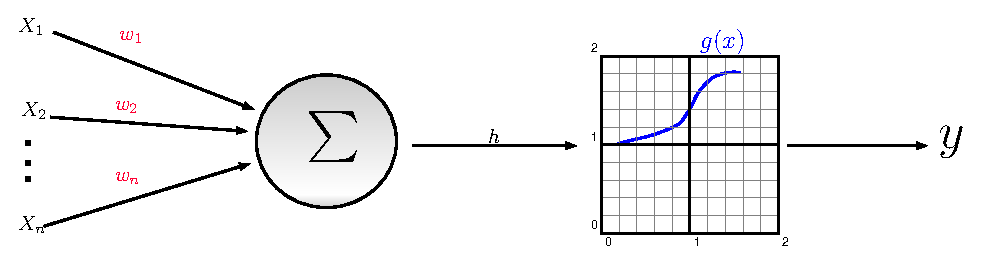
\includegraphics[scale=1]{Images/McCulloch.eps}
	}
	\caption{Modelo esquemático de um neurônio de McCulloch-Pitts. Onde $x_{1}, x_{2}, ..., x_{n}$ são os \textit{inputs}, $w_{1}, w_{2}, ..., w_{n}$ são os pesos, h é o treino, $g(x)$ é a função de ativação, e $y$ é o \textit{output}.}
	\label{Esquematico de McCulloch}
\end{figure*}

As redes alimentadas diretamente são aquelas redes cujos grafos orientados se distinguem pela presença de um ou mais camadas ocultas e cujos nós são chamados de neurônios ocultos. A função do neurônio é intervir entre a camada externa e a saída da rede de maneira útil. Adicionando-se camadas ocultas a rede torna-se capaz de realizar estatísticas de ordem elevada \citep{Haykin1999}.


\section{Resultados}

A tabela \ref{grupo01} refere-se ao conjunto de $6$ testes realizados no primeiro banco de dados que é uma composição dos dados de treinamento e testes $1$. Os testes utilizados neste trabalho foram em sua totalidade compostos por $2$ camadas ocultas. O número de neurônios ocultos estão indicados nas tabelas, como Neurônios na CO1 (camada oculta 1) e como Neurônios na CO2 (camada oculta 2).

\begin{table}[ht]
	\begin{center}
				\caption{Grupo $01$}
				\label{grupo01}
				\begin{tabular}{|c|c|c|c|c|c|c|}\hline	
					\textbf{Configuração} &\textbf{I}&\textbf{II}&\textbf{III}&\textbf{IV}&\textbf{V}&\textbf{VI} \\ \hline 
					{Neuronios na CO1} & 4 & 4 & 4 & - & 4 & 4 \\ \hline
					{Neuronios na CO2} & 4 & 4 & 2 & - & 4 & 4 \\ \hline
					{Cl. Correta (\%)} & 52.3 & 91.3 & 91.2  & - & 52.3 &  92  \\ \hline
					{Cl. Incorreta (\%)} & 47.7 & 8.7 & 8.8 & - & 47.7 & 8 \\ \hline
					{MAE (\%)} & 0.49 &  0.13 & 0.14 & - & 0.49 & 0.1363 \\ \hline
					{RMSE (\%)} & 0.50 & 0.26 & 0.27 & - & 0.49 & 0.2586 \\ \hline
					{RAE (\%)} & 99.68 & 26.23 & 28.3 & - & 100.2 & 27.3239 \\ \hline
					{RRSE(\%)} & 100.23 & 52.23 & 53.75 & - & 100.1 & 51.7764 \\ \hline
					{Dados Totais} & 1500 & 1500  & 1500 & - & 1500 & 1500 \\ \hline
				\end{tabular}  
	\end{center}
\end{table}

A tabela \ref{grupo01IV} refere-se os testes de variações de épocas do conjunto de dados $1$.

\begin{table}[ht]
	\begin{center}
		\caption{Grupo $01$: variando as épocas no teste IV}
		\label{grupo01IV}
		\begin{tabular}{|c|c|c|c|}\hline	
			\textbf{Configuração} &$\textbf{IV}_{1}$&$\textbf{IV}_{100}$&$\textbf{IV}_{1000}$ \\ \hline 
			{Neuronios na CO1}   & 4      & 4     & 4      \\ \hline
			{Neuronios na CO2}   & 4      & 4     & 4      \\ \hline
			{Cl. Correta (\%)}   & 52.3   & 90.8  & 91.53  \\ \hline
			{Cl. Incorreta (\%)} & 47.7   & 9.2   & 8.47   \\ \hline
			{MAE (\%)}           & 0.49   & 0.16  & 0.14   \\ \hline
			{RMSE (\%)}          & 0.51   & 0.27  & 0.26   \\ \hline
			{RAE (\%)}           & 99.63  & 32.34 & 27.49   \\ \hline
			{RRSE(\%)}           & 100.23 & 54.49 & 52.89  \\ \hline
			{Dados Totais}       & 1500   & 1500  & 1500   \\ \hline
		\end{tabular}  
	\end{center}
\end{table}

A Fig. \ref{grafo} apresenta a topologia da rede quando se unem os atributos semelhantes. Neste caso, o número de entradas é reduzido. Na etapa VI, nos três grupos analisados, foram unidos por meio do filtro two merge values os atributos semelhantes das classes ESTC e NDEP. Nesta exercício a classe ESTC passa a ter somente duas categorias (casado ou solteiro). E a classe NDEP passa a ter duas classes (com filhos ou sem filhos). 

\begin{figure*}[ht]
	\centering
	\setlength{\fboxsep}{8pt}
	\setlength{\fboxrule}{0.1pt}
	\fbox{
		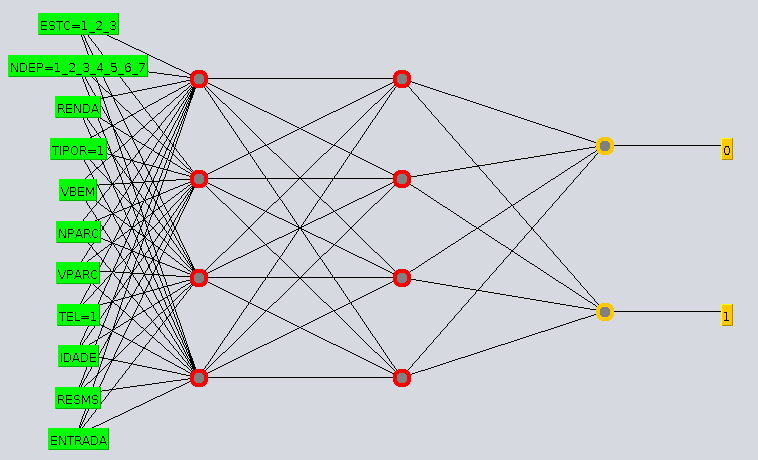
\includegraphics[scale=0.65]{Images/grafo3.png}
	}
	\caption{Grafo orientado da rede após se aplicar o filtro merge two values nas nos atributos 1,2,3,4,5,6,7 da classe NDEP e no atributos 1,2,3 da classe ESTC.}
	\label{grafo}
\end{figure*}

A tabela \ref{grupo02} apresenta o conjunto de testes para o grupo 2. 

\begin{table}[ht]
	\begin{center}
		\caption{Grupo $02$}
		\label{grupo02}
		\begin{tabular}{|c|c|c|c|c|c|c|}\hline	
			\textbf{Configuração} &\textbf{I}&\textbf{II}&\textbf{III}&\textbf{IV}&\textbf{V}&\textbf{VI} \\ \hline 
			{Neuronios na CO1} & 4 & 4 & 4 & - & 4 & 4 \\ \hline
			{Neuronios na CO2} & 4 & 4 & 8 & - & 4 & 4 \\ \hline
			{Cl. Correta (\%)} & 53.30 & 91.47 & 91.67  & - & 53.27 &  91.27 \\ \hline
			{Cl. Incorreta (\%)} & 46.7 & 8.53 & 8.33 & - & 46.73 & 8.73 \\ \hline
			{MAE (\%)} & 0.49 &  0.12 & 0.12 & - & 0.5 & 0.13 \\ \hline
			{RMSE (\%)} &0.50 & 0.26 & 0.26 & - & 0.5 & 0.27 \\ \hline
			{RAE (\%)} & 98.96 & 25.05 & 24.36 & - & 100.4 & 24.66 \\ \hline
			{RRSE(\%)} & 101.26 & 52.85 & 53.24 & - & 100.2 & 54.12 \\ \hline
			{Dados Totais} & 1500 & 1500  & 1500 & - & 1500 & 1500 \\ \hline
		\end{tabular}  
	\end{center}
\end{table}

Na tabela \ref{grupo02IV} são apresentados os subconjuntos de testes das épocas do grupo 2. 

\begin{table}[ht]
	\begin{center}
		\caption{Grupo $02$: variando as épocas no teste IV}
		\label{grupo02IV}
		\begin{tabular}{|c|c|c|c|}\hline	
			\textbf{Configuração} &$\textbf{IV}_{1}$&$\textbf{IV}_{100}$&$\textbf{IV}_{1000}$ \\ \hline 
			{Neuronios na CO1}   & 4      & 4     & 4      \\ \hline
			{Neuronios na CO2}   & 4      & 4     & 4      \\ \hline
			{Cl. Correta (\%)}   & 53.2667   & 91.4   & 91.8667  \\ \hline
			{Cl. Incorreta (\%)} & 46.7333   & 8.6    & 8.1333   \\ \hline
			{MAE (\%)}           & 0.4913   & 0.1384  & 0.1165   \\ \hline
			{RMSE (\%)}          & 0.5083   & 0.2669  & 0.2584   \\ \hline
			{RAE (\%)}           & 98.6867 & 27.807 & 23.3909   \\ \hline
			{RRSE(\%)}           & 101.8876 & 53.4966 & 51.7846  \\ \hline
			{Dados Totais}       & 1500   & 1500  & 1500   \\ \hline
		\end{tabular}  
	\end{center}
\end{table}

Na tabela \ref{grupo03} são apresentados os conjunto de testes para o grupo 3. 

\begin{table}[ht]
	\begin{center}
		\caption{Grupo $03$}
		\label{grupo03}
		\begin{tabular}{|c|c|c|c|c|c|c|}\hline	
			\textbf{Configuração} &\textbf{I}&\textbf{II}&\textbf{III}&\textbf{IV}&\textbf{V}&\textbf{VI} \\ \hline 
			{Neuronios na CO1} & 4 & 4 & 1 & - & 4 & 4 \\ \hline
			{Neuronios na CO2} & 4 & 4 & 12 & - & 4 & 4 \\ \hline
			{Cl. Correta (\%)} & 49  & 91.4  & 90.9  & - & 51 &  90 \\ \hline
			{Cl. Incorreta (\%)} & 51  & 8.6 & 9.1 & - & 49 & 10 \\ \hline
			{MAE (\%)} & 0.5 &  0.1 & 0.1 & - & 0.5  &  0.1399 \\ \hline
			{RMSE (\%)} & 0.5 & 0.2 & 0.3 & - & 0.5 &  0.2738 \\ \hline
			{RAE (\%)} & 100.1 & 24.5 & 32.7 & - & 100 & 27.986 \\ \hline
			{RRSE(\%)} & 100.3 & 53.1 & 55.6 & - & 100 & 54.7797 \\ \hline
			{Dados Totais} & 1500 & 1500  & 1500 & - & 1500 & 1500 \\ \hline
		\end{tabular}  
	\end{center}
\end{table}

A tabela \ref{grupo03IV} mostra os testes de variação das épocas do grupo 3. 

\begin{table}[ht]
	\begin{center}
		\caption{Grupo $03$: variando as épocas no teste IV}
		\label{grupo03IV}
		\begin{tabular}{|c|c|c|c|}\hline	
			\textbf{Configuração} &$\textbf{IV}_{1}$&$\textbf{IV}_{100}$&$\textbf{IV}_{1000}$ \\ \hline 
			{Neuronios na CO1}   & 4      & 4     & 4      \\ \hline
			{Neuronios na CO2}   & 4      & 4     & 4      \\ \hline
			{Cl. Correta (\%)}   & 49    & 90.3333  & 91  \\ \hline
			{Cl. Incorreta (\%)} & 51    & 9.6667   & 9   \\ \hline
			{MAE (\%)}           & 0.5002   & 0.1321  & 0.1318   \\ \hline
			{RMSE (\%)}          & 0.5004   & 0.2748  & 0.2653   \\ \hline
			{RAE (\%)}           & 100.0891  & 26.4304 & 26.3714   \\ \hline
			{RRSE(\%)}           & 100.099 & 54.9758 & 53.0768  \\ \hline
			{Dados Totais}       & 1500   & 1500  & 1500   \\ \hline
		\end{tabular}  
	\end{center}
\end{table}


Os parâmetros do modelo que permaneceram inalterados foram a taxa de aprendizado com um valor de $0.3$, momentum $0.2$, limiar de validação $20$. 


\section{Conclusões}
	Ao analisar previamente os dados é possível que o número de dependentes NDEP é majoritariamente composto por uma pessoa. 
	
	Para agrupamento 1, tabela \ref{grupo01} ,a classificação correta, quando não se utiliza a normalização é insatisfatória com uma taxa de acerto de $52.3\%$, quase muito semelhante a classificação incorreta que foi de $47.7\%$. Assim como o erro médio absoluto apresenta $49\%$ e o erro médio quadrático $50\%$, ou seja o erro está na mesma escala das medidas corretas.  Esse desempenho se deve ao fato de que a rede não consegue identificar com clareza os atributos das classes que tem escalas de valores absolutos muito discrepantes. Esse tipo de comportamento é verificado para todos os grupos 1,2 e 3, no teste I.
	
	Ainda no agrupamento 1 teste II, ao se normalizar os dados sem codificação binária dos atributos categóricos nota-se uma melhora no desempenho da rede aonde a classificação correta atinge o valor de $91.3\%$ e a incorreta $8.7\%$. O erro quadrado médio e o erro absoluto atingem respectivamente as marcas de $0.26\%$ e $0.13\%$. Esta melhora no desempenho se deve ao fato da normalização trazer para o mesmo patamar de valores os atributos de entrada facilitando o processo de classificação. Este mesmo comportamento se verificou em ambos os grupos de teste.
	
	Na tabela \ref{grupo01}, variou-se o número de neurônios ocultos da primeira camada para a última camada de $4$ para $2$. Neste teste pouca diferença foi notada e os valores de erros e acertos permaneceram constantes. Na tabela \ref{grupo02}, ao invés de diminuir o número de neurônios na camada oculta da primeira para a segunda camadas, optou-se por aumentar o número de neurônios de $4$ para $8$. Neste segundo caso de estudo os valores permaneceram praticamente inalterados. Na tabela \ref{grupo03}, aumentou-se o número de neurônios ocultos de $4$ para $12$, na segunda camada e diminuiu-se o número de neurônios ocultos de $4$ para $1$ na primeira camada. Neste caso de estudo notou-se uma piora dos índices da rede. A classificação correta caiu para $90.9\%$ e a incorreta aumentou para $9.1\%$ e os erros aumentaram. Esse aumento do erro se deve ao fato de que o arranjo topológico escolhido aglutina em um único nó oculto todos os parâmetros da rede tornando-a um mais ineficiente. Esse comportamento não se verificou nos agrupamentos $1$ e $2$.
	
	No teste IV, tabela \ref{grupo01IV}, ao se variar o número de épocas notou-se melhora nos índices da rede, subindo, por exemplo, o número de acertos de $52.3\%$ para $91.53\%$. Esse comportamento se verificou para os grupos $2$ e $3$. Isso se deve ao fato de que na primeira iteração a rede ainda não aprendeu o suficiente do banco de dados ao ponto de realizar uma classificação eficiente. Contudo, a medida que se aumentam o número de épocas para $100$ nota-se um rápido aumento de desempenho da rede. O melhor desempenho verificou-se na época $1000$, aonde os índices de classificação correta e incorreta obtiveram os melhores resultados atingindo valores de $91.53\%$ e $8.47\%$. Neste ponto a rede está totalmente treinada o que leva a um aumento expressivo no número de acertos.
	
	Com normalização dos atributos de entrada e utilizando um conjunto de validação, nota-se uma piora nos índices da rede, o que é verificado em todos os grupos de treinamento. 
	 
	Os melhores resultados foram obtidos agrupando algumas categorias das variáveis ESTC e NDEP. Para isto, utilizou-se o filtro não supervisionado \textit{Merge Two Values}. A Fig. \ref{grafo}, ilustra que o número de atributos utilizados na rede é reduzido a medida que, por exemplo, pessoas solteiras, divorciadas e viúvas, podem ser consideradas dentro da mesma categoria, a de solteiro, para uma análise bancária. Bem como o atributo número de dependentes pode ser reduzido para um filho ou nenhum filho. Estas considerações fazem com que o desempenho da rede se torne melhor impactando no número de classificações corretas atingindo o seu melhor valor de $92\%$ de acerto na tabela \ref{grupo01}.
	

% Now we need a bibliography:


\bibliographystyle{apalike}
\bibliography{references}


% Your document ends here!
\end{document}